\documentclass[10pt,openright,twoside,french]{book}
\usepackage{marvosym}
\input philippe2013
\input philippe2013_activites
\pagestyle{empty}


\begin{document}

\TitreActivite{viii.1}{Regroupement par classe}

\exo
Une étude sur la durée de vie en années de $500$ chauffe-eau fabriqués par une entreprise a donné les résultats suivants :
\begin{center}
\renewcommand\arraystretch{1.5}
    \begin{tabularx}{\linewidth}{|>{\centering\bfseries}m{3cm}|*{7}{>{\centering\arraybackslash}X|}c|}
        \hline
            Durées de vie & $\intervallefo 0 4$ & $\intervallefo 4 8$ & $\intervallefo{8}{12}$ & $\intervallefo{12}{16}$ & $\intervallefo{16}{20}$ & $\intervallefo{20}{24}$ & $\intervalleff{24}{28}$ & Total\\
        \hline
            Effectifs & $10$ & $36$ & $78$ & $120$ & $154$ & $60$ & $42$& \\
        \hline
            Centres de classe  & & & & & & && \\
        \hline
            Fréquences\par (fraction) & & & & & & & &\\
        \hline
            Fréquences (pourcentage) & & & & & & && \\
        \hline
            Fréquences Cumulées Croissantes & & & & & & && \\
        \hline
    \end{tabularx}
\end{center}

\begin{enumerate}
    \item Que signifie la troisième colonne du tableau ?
    \item Que signifie la troisième ligne du tableau ?
    \item Compléter toutes les cases vides du tableau.
    \item Calculer la durée de vie moyenne d'un chauffe-eau.
    \item Quel est le pourcentage de chauffe-eau dont la durée de vie est supérieure à $20$ ans ?
    \item Citer une différence entre un histogramme et un diagramme en bâton.
    \item Ci-dessous, tracer soigneusement le polynôme des fréquences cumulées croissantes.
    \item Utiliser le graphique de la question précédente pour déterminer une valeur approchée de la médiane de cette série ainsi que de $Q_1$ et $Q_3$.
    \item Déterminer la valeur exacte de la médiane.
\end{enumerate}\medskip

\begin{center}
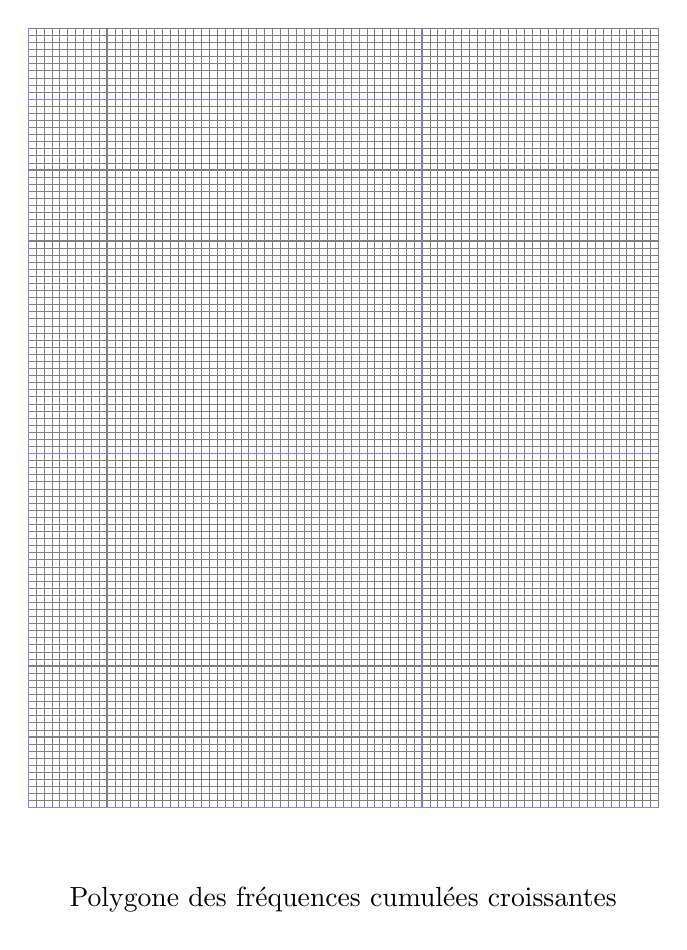
\begin{tikzpicture}[yscale=0.9]
	% Dimensions du repere
	\def\xmin{0} \def\xmax{8} \def\ymin{0} \def\ymax{11}
	% Grilles
	\draw [step=0.1,gray,very thin]  (\xmin,\ymin) grid (\xmax,\ymax);
	\draw [step=1,gray,thin] (\xmin,\ymin) grid (\xmax,\ymax);
	\draw [step=5,thin,color=blue!50]  (\xmin,\ymin) grid (\xmax,\ymax);
    \draw (4,-1.3) node {Polygone des fréquences cumulées croissantes};
\end{tikzpicture}
\end{center}

\end{document} 